%  ========================================================================
%  Copyright (c) 2022 The University of Washington
%
%  Licensed under the Apache License, Version 2.0 (the "License");
%  you may not use this file except in compliance with the License.
%  You may obtain a copy of the License at
%
%      http://www.apache.org/licenses/LICENSE-2.0
%
%  Unless required by applicable law or agreed to in writing, software
%  distributed under the License is distributed on an "AS IS" BASIS,
%  WITHOUT WARRANTIES OR CONDITIONS OF ANY KIND, either express or implied.
%  See the License for the specific language governing permissions and
%  limitations under the License.
%  ========================================================================
%

% Documentation for University of Washington thesis LaTeX document class
% by Nhut Minh Phan
% phan92@uw.edu
%
%    Revised 2020/02/24, added \caption()[]{} option.  No ToC.
%
%    Revised for version 2015/03/03 of uwthesis.cls
%    Revised, 2016/11/22, for cleanup of sample copyright and title pages
%
%    This document is contained in a single file ONLY because
%    I wanted to be able to distribute it easily.  A real thesis ought
%    to be contained on many files (e.g., one for each chapter, at least).
%
%    To help you identify the files and sections in this large file
%    I use the string '==========' to identify new files.
%
%    To help you ignore the unusual things I do with this sample document
%    I try to use the notation
%       
%    % --- sample stuff only -----
%    special stuff for my document, but you don't need it in your thesis
%    % --- end-of-sample-stuff ---


%    Printed in twoside style now that that's allowed
%
 
\documentclass [11pt, proquest] {uwthesis}[2020/02/24]
 
%
% The following line would print the thesis in a postscript font 

% \usepackage{natbib}
% \def\bibpreamble{\protect\addcontentsline{toc}{chapter}{Bibliography}}

\setcounter{tocdepth}{1}  % Print the chapter and sections to the toc
 

% ==========   Local defs and mods
%

% --- sample stuff only -----
% These format the sample code in this document

\usepackage{pgf}
\usepackage{pgfplots}
%\usepackage{url}
\usepackage{alltt}  % 
\newenvironment{demo}
  {\begin{alltt}\leftskip3em
     \def\\{\ttfamily\char`\\}%
     \def\{{\ttfamily\char`\{}%
     \def\}{\ttfamily\char`\}}}
  {\end{alltt}}
 
% metafont font.  If logo not available, use the second form
%
% \font\mffont=logosl10 scaled\magstep1
\let\mffont=\sf
% --- end-of-sample-stuff ---
 



\begin{document}
 
% ==========   Preliminary pages
%
% ( revised 2012 for electronic submission )
%

\prelimpages
 
%
% ----- copyright and title pages
%
\Title{Deep Learning Methods to Identify Intracranial Hemorrhage 
Using Tissue Pulsatility Ultrasound Imaging}
\Author{Nhut Minh Phan}
\Year{2022}
\Program{Computer Science \& Software Engineering}

\Chair{Dr. Erika Parsons}{Dr.}{Computer Science \& Software Engineering}
\Signature{Dr. Pierre Mourad}
\Signature{Dr. Michael Stiber}

\copyrightpage

\titlepage  

 
%
% ----- signature and quoteslip are gone
%

%
% ----- abstract
%


\setcounter{page}{-1}
\abstract{%
This sample dissertation is an aid to students who are attempting
to format their theses with \LaTeX, a sophisticated
text formatter widely used by mathematicians and scientists everywhere.
 
\begin{itemize}
\item It describes the use of a specialized
macro package developed specifically for thesis production
at the University.
The macros customize \LaTeX\ for the correct thesis style,
allowing the student to concentrate on the substance of
his or her text.%
\footnote{See Appendix A to obtain the source to this
 thesis and the class file.}
\item It demonstrates the solutions to a variety of
formatting challenges found in thesis production.
\item It serves as a template for a real dissertation.
\end{itemize}
}
 
%
% ----- contents & etc.
%
\tableofcontents
\listoffigures
%\listoftables  % I have no tables
 
%
% ----- glossary 
%
\chapter*{Glossary}      % starred form omits the `chapter x'
\addcontentsline{toc}{chapter}{Glossary}
\thispagestyle{plain}
%
\begin{glossary}

\item[cranium] the part of the skull that encloses the brain.
\item[CT] Computer Tomography.
\item[IED] Improvised Explosive Device.
\item[IRB] Institutional Review Board.
\item[Intracranial hemorrhage] bleeding inside the brain.
\item[TBI] Traumatic Brain Injury.
\item[TPI] Tissue Pulsatility Imaging.
\item[cTBI] closed Traumatric Brain Injury.
\item[pTBI] penetrating Traumatic Brain Injury.
\item[WHO] World Health Organization.
 
\end{glossary}
 
%
% ----- acknowledgments
%
\acknowledgments{
  I would like to express sincere appreciation to Dr. Pierre Mourad and Dr. 
  Michael Stiber for accepting my request to be on the commitee for this capstone
  project. I am also grateful for the support received from Dr. John C. Kucewicz
  and Nina LaPiana. Without their contribution in data collection, data registration,
  and signal processing, this project would not happen. Finally, I offer my very special 
  thanks to Dr. Erika Parsons for being the Chair of my committee and without whose support 
  and guidance, this project would be havebeen possible.
}

%
% ----- dedication
%
\dedication{\begin{center}To my parents, sister, and dear wife without whose support
  I would not have been able to achieve my goals.\end{center}}

%
% end of the preliminary pages
 
 
 
%
% ==========      Text pages
%

\textpages
 
% ========== Chapter 1

\chapter {Introduction}

\section{Background}

Brain injury may happen in one of two ways: close brain injury (cTBI) and penetrating 
brain injury (pTBI)\cite{TBI}. Closed brain injuries happen when an injury is nonpenetrating
and does not cause any break in the skull. The source of these injuries are rapid forward and/or
backward movements and shaking of the brain inside the bony skull that results in bruising
and tearing of brain tissue and blood vessels. Penetrating brain injuries happen when a foreign 
object penetrates the skull and then traverses through the brain parenchyma. 
For instance, a bullet travels through the head, piercing the brain.

What why is TBI important for civilians and battle field?
TBI in the battle field:
A large percentage of deployed U.S. sodiers (40\% to 60\% of surviving soldiers)
suffer from closed-head injuries caused by the blast effect of IED explosion\cite{explosive}. 
These injuries could result in intracranial hemorrhage, causing long-term neurological damages
if left untreated. For severe TBI cases, the patients must be evacuated to the nearest combat
hospital that has equipment to support neurosergery, airway protection, mechaincal ventilation,
among other means for critical care. However, severe cTBI patients often do not survive more than
one year post injury\cite{explosive}. Thus, early diagnosis is critical not only to improve the clinical 
outcome, but also to provide medical personnel with information to make decision when resources are 
scarce.

Besides the relevance on the battle field, TBI is a pressing public health and medical problem
around the world. According to the World Health Organization (WHO), TBI affects an estimate of 10 million 
people annually\cite{hyder_impact_2007}. Low and middle income countries face higher risk factors
for causes of TBI due to inadequate health care systems.

Early diagnosis and immediate medical care is extremely important in improving the clinical outcomes for 
TBI patients\cite{management_2000}. Computer Tomography (CT) and Magnetic
Resonance Imaging (MRI) are the current standard methods for identifying  intracranial 
hemorrhage\cite{heit_imaging_2017}. The main disadvantage of these imaging modalities is the
complexity, size, and cost of the required equipment, making them inaccessible in the combat settings
and in low income countries. In contrast, ultrasound imaging could be used with relatively affordable
equipment that are as small as a standard tablet. An example of such systems is a tablet-like device 
from Terason (the company website is at https://www.terason.com). Ultrasound imaging has a major
drawback: ultrasound waves do not penetrate bones very well, making ultrasound imaging more suitable
for infants up to about 18 months old at which age the craniums are yet fused together\cite{cranial_ult}.

A team of researchers from the University of Washington  developed a novel ultrasound technique called
tissue pulsatility imaging (TPI) that captures the pulsation of the brain tissue as blood infuses the
brain during a cardiac cycle\cite{kucewicz_tissue_2008}. The team collected data from civilian patients who 
suffer moderate to severe cTBI. The working hypothesis is that the difference in the movements of brain tissue versus 
TBI lesion allows one to detect intracanial hemorrhage through computer assisted means. This project aims to employ the power
of deep learning to produce an algorithm that can automatically identifying intracranial hemorrhage from TPI data.

\section{Data Collection}
The data used in this project were collected from actual humans, thus the data collection is under controlled
by the policies of the University of Washington's Human Subjects Division. Data collection was approved by 
the Institutional Review Board (IRB) through a Zipline application, the Human Subjects Division's e-IRB system.

The data was collected from patients admitted to Harborview Medical Center (HMC) in Seattle, the only Level 1 trauma 
center in the area capable of providing total care for every aspect of traumatic injuries to the brain\cite{trauma_care}.
The criteria for selecting patients are:
\begin{itemize}
  \item Moderate to severe cTBI at HMC;s Neuro ICU, with or without polytrauma
  \item Patients 18 years or older
  \item Not prisoners
  \item Not from Native American or non-U.S. indigenous populations through a tribe, tribe-focused organization, or similar community-based organization
\end{itemize}
The last two criteria are to simplify the Zipline application.
When TBI patients arrived at HMC, the patients received life saving treatment if necessary, including diagnosis of TBI via CT imaging.
A research coordinator then screened them for the inclusion criteria. If they had an injury the team is interested in, then 
the coordinator asked them or their family for consent. Ultrasound raw data were collected using a Terason (Burlington, MA) u3200t, a tablet-based, 
general purpose scanner with a 4V-2 phased array transducer (64 elements, 2.5 MHz RF sampling frequency, 128 scanlines
per frame). The scan rate was fixed by the manufacture at 30 frames per second. A certified medical sonographer used the Terason 
device in the hospital room to collect ultrasound data. Data could come from patients hours after an injury or days after 
an injury. Data collection happened after the patients were diagnosed using CT or MRI, and did not interfere or interrupt 
routine hospital clinical care.

The sonographer collected data through the temporal window of the head (See Figure \ref{ultrasound_angle}) without
shaving the head, spending approximately five minutes aiming the ultrasound toward the known intracranial hemorrhage with 
each of the following orientations: coronal, axial, and oblique. The axial is a horizontal slice of the brain at zero degree; 
coronal is a 90-degree slice of the brain; oblique is a slice at any angle from one degree to 179 degrees excluding the coronal. 
Data were collected from the left and right side of the head. The sonographer also used a pulse oximeter to capture
phases of the cardiac cycle. Any patient identifying information, including name, age, and gender, was removed from the data. 
Patients are distinguished by three-digit numbers.

Prior to restrictions imposed due to COVID-19 virus, the sonographer collected 15 scans from each side of the head equally divided between
the three scan planes. The amount of date collected following COVID-19 restriction, the data were limited to 1 axial, 1 coronal and 4 oblique
scans from each side of the head.

\begin{figure}
  \centering
  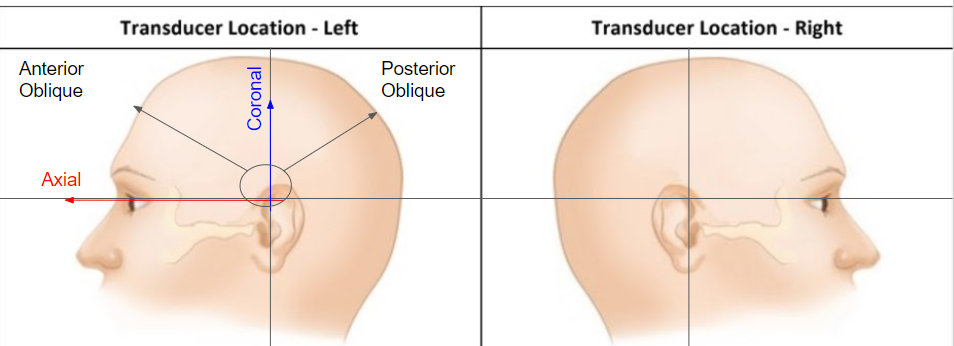
\includegraphics[width=1\linewidth]{figures/ultrasound_angle.png}
  \caption{The planes at which ultrasound data are collected: left or right side of the head and at axial, coronal, or oblique.}
  \label{ultrasound_angle}
\end{figure}

\section{Signal Processing}

Signal processing is not in the scope of my project. It was done by an ultrasound signal processing expert, Dr. John Kucewicz.
Tissue Pulsatility Imaging (TPI) relies on the deformation of the brain tissue in response to changes in 
blood volume over a cardiac cycle. During systole, blood accumulates in the tissue due to more blood entering the arterial 
vasculature than leaving leaving through the venous vasculature. The amount of tissue expansion is by a fraction of a percent.
During diastole, more blood leaves through the venous vasculature returning the tissue to presystole volume\cite{hemodynamics, pulsatile_echo}.
The central working hypothesis of the larger research effort is that this pulsation could help distinguished lesion from
healthy brain tissue. Dr. John Kucewicz works with the raw ultrasound signals from the Terason device to measure sub-micron
tissue displacement. The technique is developed based on plethysmography, an non-ultrasound method for measuring expansion of tissues
due to perfusion\cite{kucewicz_tissue_2008}.

Using well-established ultrasound signal processing techiques and the synchronization to cardiac cycles through pulse oximetry,
the raw ultrasound data were converted into displacement data (See Figure \ref{signal_processing}). At a high level, the ultrasound RF signal 
is converted into velocity of tissue movement, then into tissue displacement. First, the velocity of tissue movement was calculated from the 
frame-to-frame change in phase of the RF signal. The displacement then was calculated by taking the time integral of the velocity and 
band-pass filtered. Each scan results in an eight-second time series of tissue displacement at each pixel in a 2D image frame.

Each pixel in the ultrasound plane has a time series of tissue displacement, sampled at 30 Hz. The displacement amplitude at each pixel was 
computed by using a band pass filter in a narrow band (0.6 Hz wide) centered near the cardiac cycle frequency. A Hilbert transform is then 
applied to the narrow band filtered signal to extract the instantaneous brain displacement ampliture as a function of time. 

The process of creating masks is called registration. It entails matching the CT images for each patients obtained as part of their medical
care procedure. The team developed a procedure in MATLAB to insert and refine the placement of a 2D B-Mode data plane into a 3D CT data projection
(See Figure \ref{registration}). An example output is shown in Figure \ref{registration_output}.

\begin{figure}
  \centering
  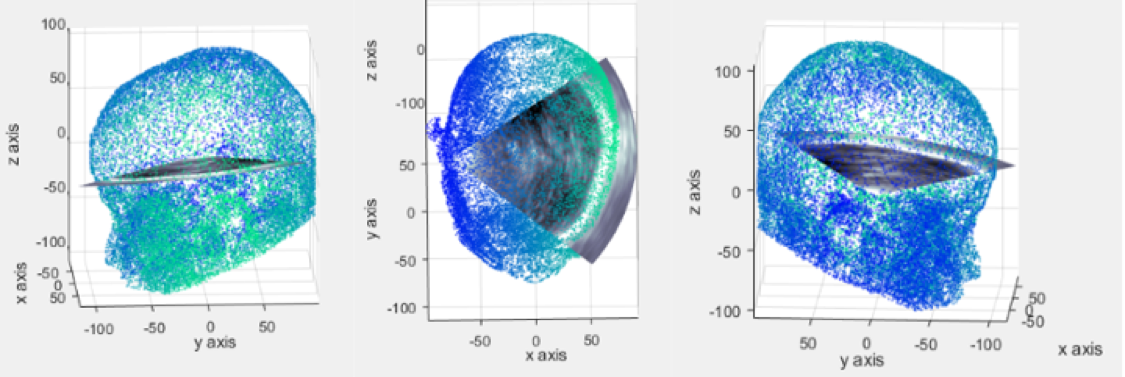
\includegraphics[width=0.9\linewidth]{figures/registration.png}
  \caption{Registering a 2D ultrasound scan plane to the 3D CT data. The 2D B-mode scane is shown relative to a point cloud representing 
  the skin surface of the head in the 3D CT data.}
  \label{registration}
\end{figure}

\begin{figure}
  \centering
  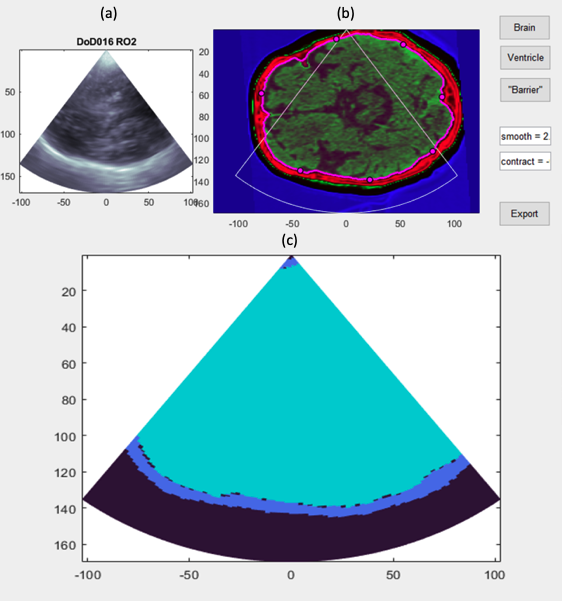
\includegraphics[width=0.7\linewidth]{figures/registration_output.png}
  \caption{CT brain mask constructed by registration with B-Mode ultrasound for patient \# 16 at the right oblique plane. 
  (a) B-mode ultrasound data. (b) An overlay of the ultrasound plane on the CT image. 
  (c) Resulting brain mask (cyan) and skull mask (blue).}
  \label{registration_output}
\end{figure}


\section{Existing System}

A previous student approached the problem of detecting intracranial hemorrhage using a different representation of 
tissue displacement data, whose description is not in the scope of this writing. The student attempted several different 
deep learning models, including MobileNetV2\cite{sandler_mobilenetv2_2019}, pix2pix\cite{isola_image_image_2018}, 
and ResNeSt\cite{zhang_resnest_2020}. The architectures of the mentioned models were used unmodified. The loss function used for model 
optimization was categorical loss entropy. The metrics used for evaluation are precision and recall. The best model 
was reported to be ResNeSt. with a reported precision score of about 0.07 and recall of about 0.2 after 70 training epochs.

The evaluation results showed that the previous deep learning methods and data preprocessing might not be suitable for the 
detection of intracranial hemorrhage from displacement data. In addition, the choice of loss function and evaluation metrics 
is poor. Categorical loss entropy considers the predicted results of all pixel an image equally. The result is that the loss 
value could be very low, but the predictive power for a class of interest is very low. The precision and recall scores evaluate 
the quantity of true positive, true negative, false positive, and false negative in relation to each other, but they do not 
indicate how well a model learn the correct label of a pixel or how well the ground truth overlaps with the detected area.

\section{Problem Statement and Scope}
This capstone project focuses on the core algorithm that detects the regions of intracranial
hemorrhage with in a patient's brain tissue. The scope is limited to data preprocessing, skull detection,
ventricle detection, brain mass detection, and intracranial hemorrhage diagnosis.

\subsection{Data Preprocessing}





\subsection{Skull Detection}


\subsection{Ventricle Detection}


\subsection{Brain Mass Detection}



\subsection{Hemorrhage Diagnosis}




% ========== Chapter 2

\chapter {Related Work}





% ========== Chapter 3

\chapter {Method}

\section{Data Description and Preprocessing}






% ========== Chapter 4

\chapter {Experiment and Result}




% ========== Chapter 5

\chapter {Conclusion and Future Work}

\section{Conclusion}



\section{Limitation}
Talk about the unique differences of bTBI and other cTBI as point out in this 
paper \cite{explosive} and that data available to the study are related to 
cTBI instead of bTBI.

From an interview with the sonographer on the team, one of the many difficulties in this
study is that the team do not know the exact time of the injury. If the more data could be
collected, she believes that it would be best if data were collected as soon as possible after
a patient is admitted. This way, the data would be "fresh", more representative of the data that
would be scanned by the medics on the battle field.


\section{Future work}


 
 
% ========== Chapter 2
 
\chapter{A Brief \\ Description of \protect\TeX}
 
The \TeX\ formatting program is the creation of
Donald Knuth of Stanford University.
It has been implemented on nearly every general purpose computer and
produces exactly the same copy on all machines.
 
\section{What is it; why is it spelled that way; 
and what do
really long section titles look like in the text and in the
Table of Contents?}
 
\TeX\ is a formatter.  A document's format is controlled
by commands embedded in the text.  
\LaTeX\ is a special version of \TeX---preloaded
with a voluminous set of macros that simplify most
formatting tasks.
 
\TeX\ uses {\it control sequences} to control
the formatting of a document.  These control sequences are usually
words or groups of letters prefaced with the backslash character
({\tt\char'134}).
For example,
Figure \ref{start-2} shows the text that printed the beginning
of this chapter.  Note the control sequence \verb"\chapter" that
instructed \TeX\ to start a new chapter, print the title, and
make an entry in the table of contents.  It is an example
of a macro defined by the \LaTeX\ macro package.
The control sequence \verb"\TeX", which prints the word \TeX,
is a standard macro from the {\it\TeX book}.
The short control sequence \verb"\\" in the title instructed \TeX\ to
break the title line at that point.
This capability is an example of an extension to \LaTeX\
provided by the uwthesis document class.
 
\begin{figure}
\begin{demo}
\uwsinglespace
\\chapter\{A Brief\\\\Description of \\TeX\}

The \\TeX\\ formatting program is the creation of
Donald Knuth of Stanford University.
\end{demo}
\label{start-2}
\caption{The beginning of the Chapter II text}
\end{figure}
 
Most of the time \TeX\ is simply building paragraphs from
text in your source files.  No control sequences are involved.
New paragraphs are indicated by a blank line in the
input file.
Hyphenation is performed automatically.
 
\section{\TeX books}
 
The primary reference for \LaTeX\ is Lamport's second edition
of the \textit{\LaTeX\ User's Guide}\cite{Lbook}.
It is easily read and should be sufficient for thesis formatting.
See also the \textsl{\LaTeX\ Companion}\cite{companion} for descriptions
of many add-on macro packages.

Although unnecessary for thesis writers, the \textsl{\TeX book}
is the primary reference for \TeX sperts worldwide.
 
\section{Mathematics}
 
The thesis class does not expand on \TeX's
or \LaTeX's
comprehensive treatment of mathematical equation printing.%
\label{c2note}\footnote{%
% a long footnote indeed.
 Although many \TeX-formatted documents contain no
 mathematics except the page numbers, it seems appropriate
 that this paper, which is in some sense about \TeX,
 ought to demonstrate an equation or two.  Here then, is a statement 
 of the {\it Nonsense Theorem}.
 
 \smallskip
 \def\RR{{\cal R\kern-.15em R}}
 {\narrower\hangindent\parindent Assume a universe $E$ and a symmetric function
  $\$$ defined on $E$, such that for each $\$^{yy}$ there exists a
  $\$^{\overline{yy}}$, where $\$^{yy} = \$^{\overline{yy}}$.
  For each element $i$ of $E$ define
  ${\cal S}(i)=\sum_i \$^{yy}+\$^{\overline{yy}}+0$.
  Then if $\RR$ is that subset of $E$ where $1+1=3$,
  for each $i$
  $$\lim_{\$\to\infty}\int {\cal S}di =
      \cases{0,&if $i\not\in\RR$;\cr
             \infty,&if $i\in\RR$.\cr}$$
  \par}} % end of the footnote
%
The {\it\TeX book}\cite{book}, {\it \LaTeX\ User's Guide}\cite{Lbook},
and {\it The \LaTeX\ Companion}\cite{companion}
thoroughly cover this topic.
 
 
\section{Languages other than English}
 
Most \LaTeX\ implementations at the University are tailored
for the English language.  However, \LaTeX\ will format many
other languages.  Unfortunately, this author has never been successful in 
learning more than a smattering of anything other than English.
Consult your department or the Tex Users Group.
\smallskip
\begin{center}
{\tt http://tug.org/},
\end{center}
\smallskip
for assistance with non-English formatting.

Unusual characters can be defined via the
font maker \hbox{\mffont METAFONT} (documented by Knuth\cite{Metafont}).
The definitions are not trivial.
Students who attempt to print a thesis with
custom fonts may soon proclaim,
 
% Note.  This is not the ideal way to print Greek
\medskip
\begin{center}
``$\mathaccent"7027\alpha\pi o\kern1pt\theta\alpha\nu\epsilon\hat\iota\nu$
\ $\theta\acute\epsilon\lambda\omega$.''
 
\end{center}
 
% ========== Chapter 3
 
\chapter{The Thesis Unformatted}
 
This chapter describes the uwthesis class (\texttt{uwthesis.cls},
version dated 2014/11/13)
in detail 
and shows how it was used to format the thesis.
A working knowledge of Lamport's \LaTeX\ manual\cite{Lbook} is assumed.
 
\section{The Control File}
 
The source to this sample thesis is a single file
only because ease of distribution was a concern.
You should not do this.  Your task will be much easier if you
break your thesis into several files:  a file for the preliminary pages,
a file for each chapter,  one for the glossary, and one for each
appendix.  Then use a control file to tie them all together.
This way you can edit and format parts of your thesis much more
efficiently.
 
Figure~\ref{control-file} shows a control file that
might have produced this thesis.
It sets the document style, with options and parameters,
and formats the various parts of the thesis---%
but contains no text of its own.
 
 
%  control file caption and figure
%
%
\begin{figure}[p]
 \begin{fullpage}
  \uwsinglespace
  \begin{verbatim}
    % LaTeX thesis control file
 
    \documentclass [11pt, proquest]{uwthesis}[2014/11/13]
 
    \begin{document}
 
    % preliminary pages
    %
    \prelimpages
    \include{prelim}
 
    % text pages
    %
    \textpages
    \include{chap1}
    \include{chap2}
    \include{chap3}
    \include{chap4}
 
    % bibliography
    %
    \bibliographystyle{plain}
    \bibliography{thesis}
 
    % appendices
    %
    \appendix
    \include{appxa}
    \include{appxb}
 
    \include{vita} 
    \end{document}
  \end{verbatim}
  \caption[A thesis control file]%
   {\narrower A thesis control file ({\tt thesis.tex}).
   This file is the input to \LaTeX\ that will produce a
   thesis.  It contains no text, only commands which
   direct the formatting of the thesis.
   }
  \label{control-file}
 \end{fullpage}
\end{figure}
 
The first section, from the \verb"\documentclass" to
the \verb"\begin{document}", defines the document class and options.
This sample thesis specifies the \texttt{proquest} style, which is now
required by the Graduate School and is the default.  
Two other, now dated, other styles are available:  \verb"twoside", which is similar but 
produces a wider binding margin and is more suitable for paper printing; and
\verb"oneside", which is really old fashoned.
This sample also specified a font size
of 11 points. 
Possible font size options are: \verb"10pt", \verb"11pt", and \verb"12pt".
Default is 12 points, which is the preference
of the Graduate School. If you choose a smaller size be sure to
check with the Graduate School for acceptability.  The smaller fonts
can produce very small sub and superscripts.

Include most additional formatting packages with \verb"\usepackage",
as describe by Lamport\cite{Lbook}.  The one exception to this
rule is the \verb"natbib" package.  Include it with the \verb"natbib"
document option.
 
Use the \verb"\includeonly" command to format only a part of your
thesis.  See Lamport\cite[sec. 4.4]{Lbook} for usage and limitations.

 
\section{The Text Pages}
 
A chapter is a major division of the thesis.  Each chapter begins
on a new page and has a Table of Contents entry.
 
\subsection{Chapters, Sections, Subsections, and Appendices}
 
 
Within the chapter title use a \verb"\\" control sequence to separate lines
in the printed title (recall Figure \ref{start-2}.).
The \verb"\\" does not affect the Table of Contents entry.
 
Format appendices just like chapters.
The control sequence \verb"\appendix" instructs \LaTeX\ to
begin using the term `Appendix' rather than `Chapter'.
 
 
Specify sections and subsections of a chapter 
with  \verb"\section" and \verb"\subsection", respectively.
In this thesis chapter and section
titles are written to the table of contents.
Consult Lamport\cite[pg. 176]{Lbook} to see which
subdivisions of the thesis can be written to the table of contents.
The \verb"\\" control sequence is not permitted in section and
subsection titles.
 
 
\subsection{Footnotes}
 
\label{footnotes}
 Footnotes format as described in the \LaTeX\ book.  You can also
 ask for end-of-chapter or end-of-thesis notes.
 The thesis class will automatically set these up if
 you ask for the document class option \texttt{chapternotes}
 or \texttt{endnotes}.  
 
If selected, chapternotes will print automatically.  If you choose
endnotes however you must explicitly indicate when to print the notes 
with the command \verb"\printendnotes".  See the style guide for
suitable endnote placement.  

\subsection{Figures and Tables}
Standard \LaTeX\ figures and tables, see Lamport\cite[sec.~C.9]{Lbook},
normally provide the most convenient means to position the figure.
Full page floats and facing captions are exceptions to this rule.

If you want a figure or table to occupy a full page enclose the
contents in a \texttt{fullpage} environment.  
See figure~\ref{facing-caption}.

\subsubsection{Facing pages}
Facing page captions are an artifact of traditional, dead-tree printing,
where a left-side (even) page faces a right-side (odd) page.

In the \texttt{twoside} style, a facing caption
is full page caption for a full page figure or table
and should face the illustration to which it refers.
You must explicitly format both pages. 
The caption part appears on an even page
(left side) and the figure or table
comes on the following odd page (right side).
Enclose the float contents for the caption 
in a \texttt{leftfullpage} environment,
and enclose the float contents for the figure or table 
in a \texttt{fullpage} environment.
The first page (left side) contains the caption. The second page
(right side) could be left blank.  A picture or graph might be pasted onto
this space. See figure~\ref{facing-caption}.


\begin{figure}[t]
\uwsinglespace
\begin{verbatim}
     \begin{figure}[p]% the left side caption
       \begin{leftfullpage}
         \caption{ . . . }
       \end{leftfullpage}
     \end{figure}
     \begin{figure}[p]% the right side space
       \begin{fullpage}
          . . .
          ( note.. no caption here )
       \end{fullpage}
     \end{figure}
\end{verbatim}
\caption[Generating a facing caption page]{This text would create a
  double page figure in the two-side styles. }
\label{facing-caption}
\end{figure}
 
You can use these commands with the \texttt{proquest} style, but they have little
effect on online viewing.
 
 
\subsection{Horizontal Figures and Tables}
Figures and tables may be formatted horizontally
(a.k.a.\ landscape) as long as their captions appear
horizontal also.  \LaTeX\ will format landscape material for you.

Include the \texttt{rotating} package 
\begin{demo}
\\usepackage[figuresright]\{rotating\}
\end{demo}
and read the documentation that comes with the package. 

Figure~\ref{sideways} is an example of how a landscape
table might be formatted. 

\begin{figure}[t]
\uwsinglespace
\begin{verbatim}
     \begin{sidewaystable}
         ...
         \caption{ . . . }
     \end{sidewaystable}
\end{verbatim}
\caption[Generating a landscape table]{This text would create a
  landscape table with caption.}
\label{sideways}
\end{figure}
 


\subsection{Figure and Table Captions}
Most captions are formatted with the \verb"\caption" macro as described 
by Lamport\cite[sec. C.9]{Lbook}. 
The uwthesis class extends this macro to allow
continued figures and tables, and to provide multiple figures and
tables with the same number, e.g., 3.1a, 3.1b, etc.
 
To format the caption for the first part of
a figure or table that cannot fit
onto a single page use the standard form:
\begin{demo}
\\caption[\textit{toc}]\{\textit{text}\}
\end{demo}
To format the caption for the subsequent parts of 
the figure or table 
use this caption:
\begin{demo}
\\caption(-)\{(continued)\}
\end{demo}
It will keep the same number and the text of the caption will be 
{\em(continued)}.

To format the caption for the first part of
a multi-part figure or table
use the format:
\begin{demo}
\\caption(a)[\textit{toc}]\{\textit{text}\}
\end{demo}
The figure or table will be lettered (with `a') as well as numbered.
To format the caption for the subsequent parts of 
the multi-part figure or table
use the format:
\begin{demo}
\\caption(\textit{x})\{\textit{text}\}
\end{demo}
where {\em x} is {\tt b}, {\tt c}, \ldots.
The parts will be lettered (with `b', `c', \ldots).

If you want a normal caption, but don't want a ToC entry:
\begin{demo}
\\caption()\{\textit{text}\}
\end{demo}
Note that the caption number will increment.  You would normally use this 
only to leave an entire chapter's captions off the ToC.


\subsection{Line spacing}

Normally line spacing will come out like it should. However, the 
ProQuest style allows single spacing in certain situations:
figure content, some lists, and etc.
Use \verb"\uwsinglespace" to switch to single spacing within
a \verb"\begin{}" and \verb"\end{}" block.
The code examples in this document does this. 

\section{The Preliminary Pages}
 
These are easy to format only because they are relatively invariant
among theses.  Therefore the difficulties have already been encountered
and overcome by \LaTeX\ and the thesis document classes.

Start with the definitions that describe your thesis.
This sample thesis was printed with the parameters:

\begin{demo}
\\Title\{The Suitability of the \\LaTeX\\ Text Formatter\\\\
   for Thesis Preparation by Technical and\\\\
   Non-technical Degree Candidates\}
\\Author\{Jim Fox\}
\\Program\{IT Infrastructure\}
\\Year\{2012\}

\\Chair\{Name of Chairperson\}\{title\}\{Chair's department\}
\\Signature\{First committee member\}
\\Signature\{Next committee member\}
\\Signature\{etc\}

\end{demo}
 
Use two or more \verb"\Chair" lines if you have co-chairs.
 
\subsection{Copyright page}
Print the copyright page with \verb"\copyrightpage".

\subsection{Title page}
Print the title page with \verb"\titlepage".
The title page of this thesis was printed with%
 
\begin{demo}
\\titlepage
\end{demo}
 
You may change default text on the title page with these
macros.  You will have to redefine \verb"\Degreetext", for instance,
if you're writing a Master's thesis instead of a dissertation.\footnote{If you use these they can
be included with the other information before \\copyrightpage".}

\begin{list}{}{\itemindent\parindent\itemsep0pt
   \def\makelabel#1{\texttt{\char`\\#1}\hfill}\uwsinglespace}
\item[Degree\char`\{{\it degree name}\char`\}]
   defaults to ``Doctor of Philosophy''
\item[School\char`\{{\it school name}\char`\}] defaults to
``University of Washington''
\item[Degreetext\char`\{{\it degree text}\char`\}] defaults to
``A dissertation submitted \ldots''
\item[textofCommittee\char`\{{\it committee label}\char`\}] defaults to
``Reading Committee:''
\item[textofChair\char`\{{\it chair label}\char`\}] defaults to
``Chair of the Supervisory Committee:''
\end{list}

These definitions must appear \underline{before} the \verb"\titlepage" command.

 
\subsection{Abstract}
Print the
abstract with \verb"\abstract".
It has one argument, which is the text of the abstract.
All the names have already been defined.
The abstract of this thesis was printed with
 
\begin{demo}
\\abstract\{This sample . . . `real' dissertation.\}
\end{demo}
 
 
\subsection{Tables of contents}
Use the standard \LaTeX\ commands to format these items.
 
 
\subsection{Acknowledgments}
Use the \verb"\acknowledgments" macro to format the acknowledgments page.
It has one argument, which is the text of the acknowledgment.
The acknowledgments of this thesis was printed with
 
\begin{demo}
\\acknowledgments\{The author wishes . . . \{\\it il miglior fabbro\}.\\par\}\}
\end{demo}
 
 
\subsection{Dedication}
Use the \verb"\dedication" macro to format the dedication page.
It has one argument, which is the text of the dedication.
 
\subsection{Vita}
Use the \verb"\vita" macro to format the curriculum vitae.
It has one argument, which chronicles your life's accomplishments.

Note that the Vita is not really a preliminary page.
It appears at the end of your thesis, just after the appendices.
 
 
%%  
%% \section{Customization of the Macros}
%%  
%% Simple customization, including 
%% alteration of default parameters,  changes to dimensions,
%% paragraph indentation, and margins, are not too difficult.
%% You have the choice of modifying the class file ({\tt uwthesis.cls})
%% or loading
%% one or more personal style files to customize your thesis.
%% The latter is usually most convenient, since you do not need
%% to edit the large and complicated class file.
%% 
 

%
% ==========   Bibliography
%
\nocite{*}   % include everything in the uwthesis.bib file
\bibliographystyle{plain}
\bibliography{uwthesis}
%
% ==========   Appendices
%
\appendix
\raggedbottom\sloppy
 
% ========== Appendix A
 
\chapter{Where to find the files}
 
The uwthesis class file, {\tt uwthesis.cls}, contains the parameter settings,
macro definitions, and other \TeX nical commands which
allow \LaTeX\ to format a thesis.  
The source to
the document you are reading, {\tt uwthesis.tex},
contains many formatting examples
which you may find useful.
The bibliography database, {\tt uwthesis.bib}, contains instructions
to BibTeX to create and format the bibliography.
You can find the latest of these files on:

\begin{itemize}
\item My page.
\begin{description}
\item[] \verb%https://staff.washington.edu/fox/tex/thesis.shtml%
\end{description}

\item CTAN
\begin{description}
\item[]  \verb%http://tug.ctan.org/tex-archive/macros/latex/contrib/uwthesis/%
\item[]  (not always as up-to-date as my site)
\end{description}

\end{itemize}

\vita{Jim Fox is a Software Engineer with IT Infrastructure Division at the University of Washington.
His duties do not include maintaining this package.  That is rather
an avocation which he enjoys as time and circumstance allow.

He welcomes your comments to {\tt fox@uw.edu}.
}


\end{document}
